% DD-PINN: Domain-Decoupled Physics-Informed Neural Networks
% Explanation document — based on Krauss et al. (2024) and Licher et al. (2025)

\documentclass[11pt]{article}

% ---------------------------------------------------------------------------
% Font and encoding
% ---------------------------------------------------------------------------
\usepackage{palatino}
\usepackage[T1]{fontenc}
\usepackage[utf8]{inputenc}

% ---------------------------------------------------------------------------
% Page layout
% ---------------------------------------------------------------------------
\usepackage[top=1in, bottom=1in, left=1.25in, right=1.25in]{geometry}
\usepackage{setspace}
\setstretch{1.1}
\setlength{\parindent}{1em}
\setlength{\parskip}{0.4em}

% ---------------------------------------------------------------------------
% Math
% ---------------------------------------------------------------------------
\usepackage{amsmath}
\usepackage{amssymb}
\usepackage{mathtools}
\usepackage{bm}

% ---------------------------------------------------------------------------
% Figures and tables
% ---------------------------------------------------------------------------
\usepackage{graphicx}
\usepackage{float}
\usepackage{booktabs}

% ---------------------------------------------------------------------------
% Colors and hyperlinks
% ---------------------------------------------------------------------------
\usepackage{xcolor}
\usepackage[colorlinks=true, linkcolor=blue!60!black, citecolor=blue!60!black, urlcolor=blue!60!black]{hyperref}
\usepackage{pdflscape}

% ---------------------------------------------------------------------------
% Lists
% ---------------------------------------------------------------------------
\usepackage{enumitem}
\setlist[itemize]{nosep, topsep=0.3em, itemsep=0.2em}

% ---------------------------------------------------------------------------
% TikZ for diagrams
% ---------------------------------------------------------------------------
\usepackage{tikz}
\usetikzlibrary{arrows.meta, positioning, calc, fit, backgrounds}

% ---------------------------------------------------------------------------
% Bibliography
% ---------------------------------------------------------------------------
\usepackage[numbers,sort&compress]{natbib}

% ---------------------------------------------------------------------------
% Custom commands
% ---------------------------------------------------------------------------
\newcommand{\R}{\mathbb{R}}
\newcommand{\xhat}{\hat{\bm{x}}}
\newcommand{\xdothat}{\dot{\hat{\bm{x}}}}
\newcommand{\avec}{\bm{a}}
\newcommand{\uvec}{\bm{u}}
\newcommand{\xvec}{\bm{x}}
\newcommand{\fssm}{\bm{f}_{\mathrm{SSM}}}
\newcommand{\fnn}{\bm{f}_{\mathrm{NN}}}
\newcommand{\phig}{\phi_g}

\title{\textbf{Domain-Decoupled Physics-Informed Neural Networks}\\[0.3em]
\large A Surrogate for Cosserat Rod Dynamics Enabling\\Real-Time Model-Predictive Control}
\author{}
\date{}

\begin{document}
\maketitle
\thispagestyle{empty}

% ===================================================================
\section{Problem Setting}
% ===================================================================

Soft continuum robots modeled by Cosserat rod theory offer compliance and dexterity, but their governing partial differential equations (PDEs) are computationally expensive to solve. A single forward simulation of the dynamic Cosserat model can take on the order of seconds, far too slow for real-time control. Model-predictive control (MPC) requires evaluating the dynamics model hundreds of times per control step, making direct use of the PDE solver infeasible.

The central problem is:
\begin{quote}
\emph{How can we replace the expensive Cosserat rod PDE solver with a neural surrogate that is fast enough for real-time MPC while remaining physically accurate?}
\end{quote}

Standard physics-informed neural networks (PINNs) partially address this, but suffer from three practical bottlenecks:
\begin{itemize}
    \item \textbf{Expensive gradient computation.} PINNs require automatic differentiation (autodiff) through the network to compute time derivatives $\partial \xhat / \partial t$, which is slow for large state spaces.
    \item \textbf{Loss balancing.} The initial condition (IC) loss, PDE residual loss, and data loss compete during training and require careful weighting schemes.
    \item \textbf{Training instability.} For complex dynamical systems with many states, PINN predictions can diverge.
\end{itemize}

The \emph{Domain-Decoupled PINN} (DD-PINN) resolves all three issues through a single architectural insight: decouple the time domain from the neural network using analytically differentiable ansatz functions.

% ===================================================================
\section{From Standard Neural Networks to Physics-Informed Neural Networks}
\label{sec:nn-vs-pinn}
% ===================================================================

To understand why PINNs exist and what DD-PINN improves upon, it is helpful to trace the progression from a standard (purely data-driven) neural network to a physics-informed one. We consider the task of learning a dynamical system:
\begin{equation}
    \dot{\xvec}(t) = \fssm(\xvec(t),\, \uvec(t)), \qquad \xvec(0) = \xvec_0,
    \label{eq:ssm}
\end{equation}
where $\xvec(t) \in \R^m$ is the state, $\uvec(t) \in \R^p$ is the input, and $\fssm$ encodes the known (but expensive) physics.

\paragraph{What is $\fssm$?} The subscript SSM stands for \emph{state-space model}. The function $\fssm$ is the mathematical representation of the physical laws that govern the system --- it is \emph{not} a neural network, but the exact (or high-fidelity) set of equations derived from first principles. For example, in a Cosserat rod model of a soft robot, $\fssm$ encodes the balance of linear and angular momentum, the constitutive (material) law, and the kinematic compatibility equations. Given the current state $\xvec$ (positions, velocities, internal forces) and input $\uvec$ (applied pressures or torques), $\fssm(\xvec, \uvec)$ returns the time derivative $\dot{\xvec}$ --- i.e., how the state changes in the next instant. Computing $\fssm$ is typically cheap for a single evaluation; what is expensive is \emph{integrating} it forward in time over many small steps to obtain a full trajectory, which is what the PDE solver does.

\subsection{Step 1: Standard Neural Network (Data-Driven)}

A standard neural network treats the dynamical system as a black-box regression problem. It learns a mapping from inputs to outputs using \emph{only} observed data, with no knowledge of the governing equations.

\paragraph{Setup.} Collect a dataset of $N$ state trajectories from the simulator:
\begin{equation}
    \mathcal{D} = \big\{ (\xvec_0^{(i)},\, \uvec^{(i)},\, t^{(i)},\, \xvec^{(i)}_{\mathrm{true}}) \big\}_{i=1}^{N}.
\end{equation}

\paragraph{Architecture.} A feedforward network $\bm{h}_\theta$ maps inputs directly to the predicted state:
\begin{equation}
    \xhat_t = \bm{h}_\theta(\xvec_0,\, \uvec,\, t).
\end{equation}

\paragraph{Loss function.} Training minimizes the mean squared error between predictions and data:
\begin{equation}
    \mathcal{L}_{\mathrm{data}}(\theta) = \frac{1}{N} \sum_{i=1}^{N} \left\| \bm{h}_\theta(\xvec_0^{(i)},\, \uvec^{(i)},\, t^{(i)}) - \xvec^{(i)}_{\mathrm{true}} \right\|^2.
    \label{eq:nn-loss}
\end{equation}

\paragraph{Key properties.}
\begin{itemize}
    \item The network knows \emph{nothing} about the physics --- it treats the data as arbitrary input-output pairs.
    \item Predictions can violate conservation laws, produce non-physical states, or diverge outside the training distribution.
    \item Requires \emph{large} datasets to generalize, because the network must learn the physics implicitly from examples alone.
\end{itemize}

\subsection{Step 2: Adding Physics to the Loss (PINN)}

The key idea of Raissi et al.~\cite{Raissi2019} is to \textbf{embed the known governing equations directly into the training loss}. The network architecture is identical --- what changes is \emph{how} it is trained.

\paragraph{Architecture.} The same feedforward network:
\begin{equation}
    \xhat_t = \bm{h}_\theta(\xvec_0,\, \uvec,\, t).
\end{equation}

\paragraph{Physics residual.} Since we know the governing equation $\dot{\xvec} = \fssm(\xvec, \uvec)$, we can check whether the network's prediction \emph{obeys} it. At any point $t$, compute the residual:
\begin{equation}
    \bm{r}(t) = \frac{\partial \xhat_t}{\partial t} - \fssm(\xhat_t,\, \uvec_t).
    \label{eq:residual}
\end{equation}
If the prediction is physically correct, this residual is zero everywhere. The derivative $\partial \xhat_t / \partial t$ is obtained via \textbf{automatic differentiation} (autodiff) of the network output with respect to its input $t$.

\paragraph{What is automatic differentiation?} Automatic differentiation (autodiff) is the mechanism that deep learning frameworks such as PyTorch and TensorFlow use to compute derivatives. When a neural network computes its output, the framework records every arithmetic operation in a \emph{computational graph}. To find a derivative --- for instance $\partial \xhat_t / \partial t$ --- the framework walks backward through this graph, applying the chain rule at each node. This is exact (not a finite-difference approximation) and works for arbitrarily complex networks.

In a standard neural network, autodiff is used only to compute $\partial \mathcal{L} / \partial \theta$ (the gradient of the loss with respect to the network weights $\theta$) for gradient descent. A PINN requires an \emph{additional} use of autodiff: computing $\partial \xhat_t / \partial t$ (the derivative of the output with respect to the \emph{input} $t$). This second pass through the computational graph adds significant cost, especially for large networks and many collocation points, because the entire graph must be retained and traversed for each evaluation. This is the computational bottleneck that DD-PINN eliminates by replacing autodiff-based time derivatives with closed-form analytical expressions.

\paragraph{Collocation points.} The residual~\eqref{eq:residual} is evaluated at $N_c$ randomly sampled time points $\{t_k\}_{k=1}^{N_c}$ called \emph{collocation points}. These require no simulation data --- they are points where we \emph{demand} the physics hold.

\paragraph{Loss function.} The PINN loss combines three terms:
\begin{equation}
    \mathcal{L}(\theta) = \underbrace{\lambda_1 \left\| \xhat_0 - \xvec_0 \right\|^2}_{\substack{\mathcal{L}_{\mathrm{IC}} \\ \text{initial condition}}}
    + \underbrace{\lambda_2 \frac{1}{N_c}\sum_{k=1}^{N_c} \left\| \frac{\partial \xhat_{t_k}}{\partial t} - \fssm(\xhat_{t_k}, \uvec_{t_k}) \right\|^2}_{\substack{\mathcal{L}_{\mathrm{phys}} \\ \text{physics residual at collocation points}}}
    + \underbrace{\lambda_3 \frac{1}{N_d}\sum_{k=1}^{N_d} \left\| \xhat_{t_k} - \xvec_{\mathrm{data},k} \right\|^2}_{\substack{\mathcal{L}_{\mathrm{data}} \\ \text{observed data (optional)}}}.
    \label{eq:pinn-loss}
\end{equation}

The weights $\lambda_1, \lambda_2, \lambda_3$ balance the three objectives.

\paragraph{Key properties.}
\begin{itemize}
    \item The physics loss acts as a \emph{regularizer}: even with little data, the network is steered toward physically consistent solutions.
    \item The initial condition loss $\mathcal{L}_{\mathrm{IC}}$ ensures the prediction starts at the correct state.
    \item The data loss $\mathcal{L}_{\mathrm{data}}$ is optional --- a PINN can be trained with \emph{zero} observed data if the physics are fully known.
    \item Collocation points are free (no simulation needed), so physics supervision scales cheaply.
\end{itemize}

\subsection{Step 3: Side-by-Side Comparison}

Table~\ref{tab:nn-vs-pinn} summarizes the differences.

\begin{table}[H]
\centering
\caption{Standard neural network vs.\ physics-informed neural network (PINN).}
\label{tab:nn-vs-pinn}
\begin{tabular}{@{}p{3.8cm}p{5cm}p{5cm}@{}}
\toprule
\textbf{Aspect} & \textbf{Standard NN} & \textbf{PINN} \\
\midrule
Knowledge of physics & None & Governing equations embedded in loss \\
\addlinespace[0.3em]
Loss function & $\mathcal{L}_{\mathrm{data}}$ only & $\mathcal{L}_{\mathrm{IC}} + \mathcal{L}_{\mathrm{phys}} + \mathcal{L}_{\mathrm{data}}$ \\
\addlinespace[0.3em]
Training data required & Large (must learn physics from examples) & Small or zero (physics provides supervision) \\
\addlinespace[0.3em]
Generalization & Poor outside training distribution & Better --- physics constrains extrapolation \\
\addlinespace[0.3em]
Physical consistency & Not guaranteed & Enforced at collocation points \\
\addlinespace[0.3em]
Gradient computation & Standard backprop (w.r.t.\ $\theta$ only) & Backprop w.r.t.\ $\theta$ \emph{and} autodiff w.r.t.\ input $t$ \\
\addlinespace[0.3em]
Training cost & Low per epoch & Higher (autodiff for $\partial \xhat / \partial t$) \\
\addlinespace[0.3em]
Loss balancing & Single loss --- no balancing needed & Three competing losses --- requires tuning $\lambda_1, \lambda_2, \lambda_3$ \\
\bottomrule
\end{tabular}
\end{table}

\subsection{Step 4: What DD-PINN Changes}

The DD-PINN (Section~\ref{sec:ddpinn}) keeps the PINN's core insight --- embedding physics into the loss --- but restructures the architecture to eliminate its two main costs: autodiff for time derivatives and loss balancing for the initial condition. The progression is:

\begin{enumerate}
    \item \textbf{Standard NN:} learns $\xhat_t = \bm{h}_\theta(\xvec_0, \uvec, t)$ from data only.
    \item \textbf{PINN:} same architecture, but adds $\mathcal{L}_{\mathrm{IC}} + \mathcal{L}_{\mathrm{phys}}$ to the loss. Requires autodiff w.r.t.\ $t$.
    \item \textbf{DD-PINN:} network outputs ansatz parameters $\avec = \fnn(\xvec_0, \uvec;\, \theta)$; time enters only through the analytical ansatz $\bm{g}(\avec, t)$. No autodiff for $t$; IC satisfied exactly.
\end{enumerate}

% ===================================================================
\section{PINN Loss in Detail}
% ===================================================================

For reference, the full PINN loss from Eq.~\eqref{eq:pinn-loss} is restated here with annotation. The physics loss $\mathcal{L}_{\mathrm{phys}}$ is evaluated at collocation points $(t_k)$ sampled over the prediction horizon. Computing $\partial \xhat_t / \partial t$ requires backpropagating through the network with respect to the input $t$ --- this is the computational bottleneck that DD-PINN eliminates.

% ===================================================================
\section{The DD-PINN Method}
\label{sec:ddpinn}
% ===================================================================

\subsection{Core Idea: Domain Decoupling}

The key insight is to \textbf{remove time as a network input} and instead let the network output the parameters of a pre-defined, analytically differentiable \emph{ansatz function} $\bm{g}(\avec, t)$.

\paragraph{What is an ansatz?} The word \emph{ansatz} (German for ``approach'' or ``initial placement'') is a standard term in physics and mathematics for a \textbf{guessed functional form} of the solution. Rather than solving a problem from scratch, one proposes that the answer has a specific structure --- for example, ``the solution is a sum of sinusoids with unknown amplitudes and frequencies'' --- and then determines the unknown parameters by substituting the ansatz into the governing equations. An ansatz is \emph{not} learned; it is chosen by the designer based on physical intuition about what kind of functions the solution might resemble. The power of an ansatz is that it reduces a hard problem (find an arbitrary function) to an easier one (find a finite set of parameters within a known functional form).

In the DD-PINN, the ansatz $\bm{g}(\avec, t)$ is a sum of sinusoidal basis functions (Eq.~\ref{eq:ansatz}). The neural network's job is to predict the parameters $\avec$ (amplitudes, frequencies, phases) of this ansatz for each given initial condition. Because the ansatz has a known analytical form, its time derivative $\dot{\bm{g}}$ can be written down directly --- no automatic differentiation is needed.

\medskip
\noindent The predicted state becomes:
\begin{equation}
    \boxed{\xhat_t = \bm{g}(\avec, t) + \xvec_0, \qquad \avec = \fnn(\xvec_0, \uvec_0;\, \theta)}
    \label{eq:ddpinn-core}
\end{equation}
where $\fnn$ is a feedforward neural network with parameters $\theta$, and $\avec$ is the parameter vector it outputs.

The ansatz $\bm{g}$ must satisfy two properties:
\begin{enumerate}
    \item \textbf{Differentiable in closed form} for all $t \in [0, T_s]$, so $\dot{\bm{g}}(\avec, t)$ can be computed analytically.
    \item \textbf{Zero at $t = 0$}: $\bm{g}(\avec, 0) \equiv \bm{0}$, which guarantees $\xhat_0 = \xvec_0$ exactly.
\end{enumerate}

This decoupling has three immediate consequences:
\begin{itemize}
    \item Time derivatives are computed \emph{analytically} --- no autodiff through the network.
    \item The initial condition is satisfied \emph{by construction} --- $\mathcal{L}_{\mathrm{IC}} \equiv 0$.
    \item The network is called \emph{once} per prediction, then the ansatz is evaluated at any number of collocation points cheaply.
\end{itemize}

\subsection{Ansatz Function}

For each state variable $j \in \{1, \ldots, m\}$, the ansatz is a sum of $n_g$ basis functions:
\begin{equation}
    g_j(t) = \sum_{i=1}^{n_g} \alpha_{ij} \Big[ \phig(\beta_{ij}\, t + \gamma_{ij}) - \phig(\gamma_{ij}) \Big],
    \label{eq:ansatz}
\end{equation}
where $\phig(x) = \sin(x)$ is the base construction function. The subtraction $\phig(\gamma_{ij})$ ensures $g_j(0) = 0$. The neural network outputs the parameter vector:
\begin{equation}
    \avec = \begin{pmatrix} \bm{\alpha} \\ \bm{\beta} \\ \bm{\gamma} \end{pmatrix} \in \R^{3 \cdot m \cdot n_g}.
    \label{eq:param-vector}
\end{equation}

Each parameter has an interpretable role:
\begin{itemize}
    \item $\alpha_{ij}$: amplitude of the $i$-th basis for state $j$,
    \item $\beta_{ij}$: frequency,
    \item $\gamma_{ij}$: phase offset.
\end{itemize}

An optional damping variant adds exponential decay:
\begin{equation}
    g_j^{(\mathrm{d})}(t) = \sum_{i=1}^{n_g} \alpha_{ij}\, e^{-\delta_{ij} t} \Big[ \phig(\beta_{ij}\, t + \gamma_{ij}) - \phig(\gamma_{ij}) \Big],
    \label{eq:ansatz-damped}
\end{equation}
with an additional parameter $\delta_{ij} \geq 0$ per basis, expanding the output to $\avec \in \R^{4 \cdot m \cdot n_g}$.

\subsection{Closed-Form Gradients}

The time derivative of the predicted state is computed analytically:
\begin{equation}
    \frac{\partial \xhat_t}{\partial t} = \dot{\bm{g}}(\avec, t), \qquad
    \dot{g}_j(t) = \sum_{i=1}^{n_g} \alpha_{ij}\, \beta_{ij}\, \cos(\beta_{ij}\, t + \gamma_{ij}).
    \label{eq:closed-form-grad}
\end{equation}

For the damped variant:
\begin{equation}
    \dot{g}_j^{(\mathrm{d})}(t) = \sum_{i=1}^{n_g} \alpha_{ij}\, e^{-\delta_{ij} t} \Big[ \beta_{ij}\, \cos(\beta_{ij}\, t + \gamma_{ij}) - \delta_{ij}\, \sin(\beta_{ij}\, t + \gamma_{ij}) \Big].
    \label{eq:closed-form-grad-damped}
\end{equation}

These are elementary operations --- no computational graph is constructed, and the cost scales linearly with $n_g \cdot m$ regardless of network depth.

\subsection{Loss Function}

Since $\mathcal{L}_{\mathrm{IC}} \equiv 0$ by construction, the training loss simplifies to:
\begin{equation}
    \mathcal{L}(\theta) = \lambda_{\mathrm{phys}}\, \mathcal{L}_{\mathrm{phys}}(\theta) + \lambda_{\mathrm{data}}\, \mathcal{L}_{\mathrm{data}}(\theta),
    \label{eq:ddpinn-loss}
\end{equation}
where:
\begin{align}
    \mathcal{L}_{\mathrm{phys}} &= \frac{1}{N_c} \sum_{k=1}^{N_c} \left\| \dot{\bm{g}}(\avec, t_k) - \fssm(\xhat_{t_k},\, \uvec_{t_k}) \right\|^2, \label{eq:phys-loss} \\
    \mathcal{L}_{\mathrm{data}} &= \frac{1}{N_d} \sum_{k=1}^{N_d} \left\| \xhat_{t_k} - \xvec_{\mathrm{data},k} \right\|^2, \label{eq:data-loss}
\end{align}
with $N_c$ collocation points for the physics loss and $N_d$ data points. Because gradient evaluation is cheap, DD-PINN uses 10--25$\times$ more collocation points than standard PINNs, improving physics enforcement.

\subsection{Higher-Order Excitation Inputs}

Standard PINNs assume a zero-order hold on the input $\uvec_t = \uvec_0$ over the prediction interval. DD-PINN supports polynomial interpolation:
\begin{align}
    \text{Zero-order ($\delta_u = 0$):} &\quad \uvec_t = \uvec_0, \\
    \text{First-order ($\delta_u = 1$):} &\quad \uvec_t = (1 - t_*)\, \uvec_0 + t_*\, \uvec_T, \quad t_* = t/T_s, \\
    \text{Second-order ($\delta_u = 2$):} &\quad \uvec_t = (2\uvec_0 - 4\uvec_{T/2} + 2\uvec_T)\, t_*^2 + (-3\uvec_0 + 4\uvec_{T/2} - \uvec_T)\, t_* + \uvec_0.
\end{align}

Higher-order interpolation allows smoother control trajectories within each MPC step.

% ===================================================================
\section{Architecture Overview}
% ===================================================================

Figure~\ref{fig:architecture} illustrates the DD-PINN inference pipeline.

\begin{figure}[H]
\centering
\resizebox{\textwidth}{!}{%
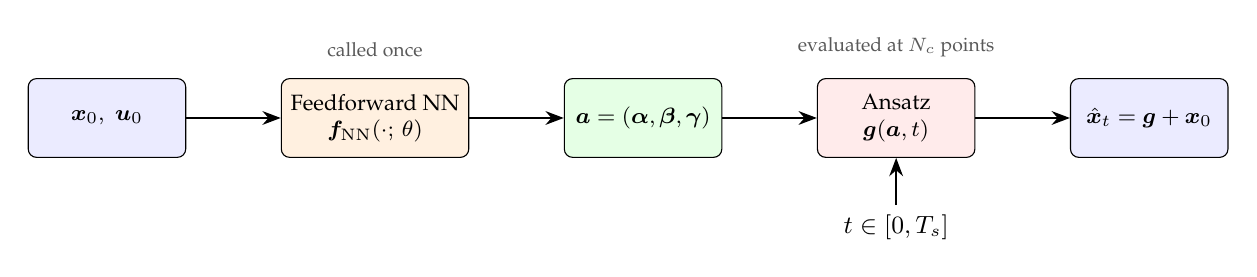
\begin{tikzpicture}[
    >=Stealth,
    block/.style={draw, rounded corners=3pt, minimum height=1cm, minimum width=2cm,
                  align=center, font=\footnotesize},
    arrow/.style={->, thick},
    label/.style={font=\scriptsize, text=gray!70!black}
]
    % Input
    \node[block, fill=blue!8] (input) {$\xvec_0,\; \uvec_0$};

    % NN
    \node[block, fill=orange!12, right=1.2cm of input] (nn) {Feedforward NN\\$\fnn(\cdot;\, \theta)$};

    % Parameters
    \node[block, fill=green!10, right=1.2cm of nn] (params) {$\avec = (\bm{\alpha}, \bm{\beta}, \bm{\gamma})$};

    % Ansatz
    \node[block, fill=red!8, right=1.2cm of params] (ansatz) {Ansatz\\$\bm{g}(\avec, t)$};

    % Output
    \node[block, fill=blue!8, right=1.2cm of ansatz] (output) {$\xhat_t = \bm{g} + \xvec_0$};

    % Time input to ansatz
    \node[below=0.6cm of ansatz, font=\small] (time) {$t \in [0, T_s]$};

    % Arrows
    \draw[arrow] (input) -- (nn);
    \draw[arrow] (nn) -- (params);
    \draw[arrow] (params) -- (ansatz);
    \draw[arrow] (ansatz) -- (output);
    \draw[arrow] (time) -- (ansatz);

    % Labels
    \node[label, above=0.15cm of nn] {called once};
    \node[label, above=0.15cm of ansatz] {evaluated at $N_c$ points};
\end{tikzpicture}}
\caption{DD-PINN inference. The neural network is evaluated once per prediction to produce ansatz parameters $\avec$. The ansatz $\bm{g}(\avec, t)$ is then evaluated at arbitrarily many time points without additional network calls.}
\label{fig:architecture}
\end{figure}

\noindent\textbf{Network details.} The feedforward network $\fnn$ uses:
\begin{itemize}
    \item \textbf{Inputs:} initial state $\xvec_0 \in \R^m$, excitation $\uvec_0 \in \R^p$ (optionally with future input samples for higher-order interpolation).
    \item \textbf{Hidden layers:} 1--4 fully connected layers with 64--128 neurons and GELU activations.
    \item \textbf{Output:} parameter vector $\avec \in \R^{3 m n_g}$ (or $\R^{4 m n_g}$ with damping).
\end{itemize}

% ===================================================================
\section{Application: Cosserat Rod Dynamics}
\label{sec:cosserat}
% ===================================================================

\subsection{Governing Equations}

A soft continuum robot is modeled as a Cosserat rod with 12 coupled PDEs in local-frame formulation (LFF):
\begin{equation}
    \xvec(s, t) = \begin{pmatrix} \xvec_1(s,t) \\ \xvec_2(s,t) \end{pmatrix} \in \R^{12},
\end{equation}
where $\xvec_1$ contains local linear and angular velocities, and $\xvec_2$ contains internal strains related to forces and moments through the compliance relation $\xvec_2 = \bm{C}^{-1} \bm{\varepsilon}$. A Kelvin--Voigt damping model adds viscous terms via damping matrix $\bm{D}_u$.

\subsection{Spatial Discretization}

The spatial domain is discretized using the implicit midpoint rule at $n_n$ collocation nodes, yielding a state-space model:
\begin{equation}
    \dot{\xvec} = \bm{f}(\xvec, \uvec, \bm{\theta}^{\mathrm{cr}}), \qquad \xvec \in \R^{72},\quad \uvec \in \R^3,
    \label{eq:cosserat-ssm}
\end{equation}
where $\xvec$ contains $12(n_n - 1) + 12 = 72$ discrete states (including end-cap boundary conditions) and $\uvec = (p_1, p_2, p_3)^\top$ represents three pneumatic chamber pressures. The parameter vector $\bm{\theta}^{\mathrm{cr}}$ includes material properties such as bending compliance.

This is the largest state-space model (72 states) learned by a physics-informed neural network for robot control to date.

\subsection{DD-PINN as Surrogate}

The DD-PINN learns the mapping $(\xvec_0, \uvec_0) \mapsto \avec$ such that $\bm{g}(\avec, t) + \xvec_0$ approximates the solution of~\eqref{eq:cosserat-ssm} over one time step $T_s$. Training data is generated from a symbolic computer algebra system (CAS) implementation of the Cosserat rod model, providing exact Jacobians for efficient data generation.

\subsection{Integration into MPC}

The DD-PINN surrogate is embedded in a nonlinear evolutionary MPC (NEMPC):

\begin{enumerate}
    \item At each control step, the MPC optimizes a sequence of future inputs $\uvec_{0:H}$ over a horizon $H$.
    \item For each candidate input sequence, the DD-PINN predicts the state trajectory by iterating one-step predictions.
    \item The optimizer selects the input sequence minimizing a cost (e.g., end-effector tracking error).
    \item Only the first input is applied; the process repeats at the next step.
\end{enumerate}

The DD-PINN achieves a \textbf{44,000$\bm{\times}$ speedup} over the full Cosserat rod solver, enabling MPC execution at \textbf{70\,Hz on GPU}.

\subsection{State Estimation via UKF}

An unscented Kalman filter (UKF) uses the DD-PINN as its state-transition model to estimate:
\begin{itemize}
    \item The full 72-dimensional internal state from partial observations (e.g., end-effector position only).
    \item The bending compliance parameter $\bm{\theta}^{\mathrm{cr}}$ online, compensating for model inaccuracies and material aging.
\end{itemize}

% ===================================================================
\section{Comprehensive Comparison of Four Approaches}
\label{sec:four-way}
% ===================================================================

Table~\ref{tab:four-way} compares four approaches for predicting the dynamics of a system governed by known PDEs: the classical PDE solver, a purely data-driven neural network, a standard PINN, and the DD-PINN.

\begin{landscape}

\begin{table}[H]
\centering
\caption{Comparison of four approaches --- formulation and training.}
\label{tab:four-way-a}
\footnotesize
\renewcommand{\arraystretch}{1.2}
\begin{tabular}{@{} p{2.8cm} p{4.2cm} p{4.2cm} p{4.2cm} p{4.2cm} @{}}
\toprule
\textbf{Aspect}
    & \textbf{PDE Solver}
    & \textbf{Standard NN}
    & \textbf{PINN}
    & \textbf{DD-PINN} \\
\midrule

\textbf{Core idea}
    & Numerically integrate the governing PDEs
    & Learn input$\to$output from data only
    & Learn input$\to$output with PDE residual in loss
    & Learn ansatz parameters; time enters analytically \\

\textbf{Physics knowledge}
    & Full (equations solved exactly)
    & None
    & Embedded in loss ($\mathcal{L}_{\mathrm{phys}}$)
    & Embedded in loss ($\mathcal{L}_{\mathrm{phys}}$) \\

\textbf{Training data}
    & Not applicable
    & Large dataset required
    & Small or zero (physics supervises)
    & Small or zero \\

\textbf{Prediction}
    & $\xvec_t = \text{ODE/PDE solve}$
    & $\xhat_t = \bm{h}_\theta(\xvec_0, \uvec, t)$
    & $\xhat_t = \bm{h}_\theta(\xvec_0, \uvec, t)$
    & $\xhat_t = \bm{g}(\fnn(\xvec_0,\uvec;\theta),\, t) + \xvec_0$ \\

\textbf{Time handling}
    & Stepwise numerical integration
    & Network input
    & Network input
    & Ansatz argument (not a network input) \\

\textbf{Time derivative}
    & Finite differences / implicit solve
    & Not computed
    & Autodiff w.r.t.\ $t$ (expensive)
    & Closed-form $\dot{\bm{g}}(\avec, t)$ (cheap) \\

\textbf{Loss function}
    & N/A
    & $\mathcal{L}_{\mathrm{data}}$
    & $\mathcal{L}_{\mathrm{IC}} + \mathcal{L}_{\mathrm{phys}} + \mathcal{L}_{\mathrm{data}}$
    & $\mathcal{L}_{\mathrm{phys}} + \mathcal{L}_{\mathrm{data}}$ \\

\textbf{Loss balancing}
    & N/A
    & 1 term --- none needed
    & 3 terms ($\lambda_1, \lambda_2, \lambda_3$)
    & 2 terms ($\lambda_{\mathrm{phys}}, \lambda_{\mathrm{data}}$) \\

\textbf{Initial condition}
    & Exact (boundary condition)
    & Not enforced
    & Via loss penalty $\mathcal{L}_{\mathrm{IC}}$ (approximate)
    & Exact by construction ($\bm{g}(\avec,0) \equiv \bm{0}$) \\

\bottomrule
\end{tabular}
\end{table}

\begin{table}[H]
\centering
\caption{Comparison of four approaches --- performance and practical aspects.}
\label{tab:four-way-b}
\footnotesize
\renewcommand{\arraystretch}{1.2}
\begin{tabular}{@{} p{2.8cm} p{4.2cm} p{4.2cm} p{4.2cm} p{4.2cm} @{}}
\toprule
\textbf{Aspect}
    & \textbf{PDE Solver}
    & \textbf{Standard NN}
    & \textbf{PINN}
    & \textbf{DD-PINN} \\
\midrule

\textbf{Physical consistency}
    & Exact (up to discretization)
    & Not guaranteed
    & Enforced at collocation points
    & Enforced at collocation points \\

\textbf{Inference speed}
    & Slow ($\sim$seconds/step)
    & Fast ($\sim\!\mu$s)
    & Fast ($\sim\!\mu$s)
    & Fast ($\sim\!\mu$s) \\

\textbf{Training cost}
    & N/A
    & Low
    & High (autodiff overhead)
    & Medium ($5$--$38\times$ faster than PINN) \\

\textbf{Collocation points}
    & N/A
    & N/A
    & $\sim$20k--40k
    & $\sim$250k--1M (cheap to evaluate) \\

\textbf{Generalization}
    & Exact for any valid input
    & Poor outside training distribution
    & Good (physics constrains extrapolation)
    & Good (physics constrains extrapolation) \\

\textbf{Stability}
    & Depends on integrator
    & Can overfit or diverge
    & Can diverge for $m \gg 1$
    & Stable (demonstrated for $m = 72$) \\

\textbf{Speedup vs.\ solver}
    & $1\times$ (baseline)
    & $\sim$10k--100k$\times$
    & $\sim$10k--100k$\times$
    & $\sim$44,000$\times$ (demonstrated) \\

\textbf{Real-time MPC}
    & No (too slow)
    & Yes (but no physics guarantees)
    & Yes
    & Yes (70\,Hz demonstrated) \\

\textbf{Key limitation}
    & Computational cost
    & Needs large data; no physics guarantees
    & Autodiff cost; loss balancing; IC approximate
    & Ansatz must be designed a priori \\

\bottomrule
\end{tabular}
\end{table}

\end{landscape}

\paragraph{Summary.} The four methods represent a spectrum from exact physics (PDE solver) to pure data (standard NN), with PINNs and DD-PINNs occupying the middle ground. The DD-PINN preserves the PINN's physics-informed training while eliminating its two main engineering costs: expensive autodiff for time derivatives and the need to balance three competing loss terms. The result is a surrogate that trains faster, satisfies initial conditions exactly, and scales to large state spaces where standard PINNs become unstable.

% ===================================================================
\section{Results Summary}
% ===================================================================

\begin{table}[H]
\centering
\caption{DD-PINN performance on dynamic Cosserat rod control.}
\label{tab:results}
\begin{tabular}{@{}ll@{}}
\toprule
\textbf{Metric} & \textbf{Value} \\
\midrule
State dimension & 72 \\
Input dimension & 3 (pneumatic pressures) \\
Speedup over full solver & 44,000$\times$ \\
End-effector error & $<\!3$\,mm ($2.3\%$ of actuator length) \\
MPC frequency & 70\,Hz (GPU) \\
Real-world acceleration & up to 3.55\,m/s$^2$ \\
Training convergence & $8.7\times$ faster than PINC (average) \\
\bottomrule
\end{tabular}
\end{table}

% ===================================================================
\section{Limitations}
% ===================================================================

\begin{itemize}
    \item \textbf{No external forces.} The current formulation neglects external forces (gravity, contact, friction), limiting applicability to free-space operation.
    \item \textbf{Pneumatic actuation only.} Inputs are chamber pressures; adapting to other actuation types (e.g., tendon-driven, rest curvature) requires reformulating the input space.
    \item \textbf{No public code.} As of early 2026, no open-source implementation is available.
    \item \textbf{Single-step prediction.} Autoregressive rollout over many steps may accumulate errors, though the MPC framework mitigates this via feedback.
\end{itemize}

% ===================================================================
\section*{References}
% ===================================================================

\begingroup
\renewcommand{\section}[2]{}  % suppress "References" heading from natbib
\begin{thebibliography}{9}

\bibitem{Raissi2019}
M.~Raissi, P.~Perdikaris, and G.~E.~Karniadakis,
``Physics-informed neural networks: A deep learning framework for solving forward and inverse problems involving nonlinear partial differential equations,''
\emph{Journal of Computational Physics}, vol.~378, pp.~686--707, 2019.

\bibitem{Krauss2024}
H.~Krauss, T.-L.~Habich, M.~Bartholdt, T.~Seel, and M.~Schappler,
``Domain-decoupled physics-informed neural networks with closed-form gradients for fast model learning of dynamical systems,''
\emph{arXiv:2408.14951}, 2024.

\bibitem{Licher2025}
J.~Licher, M.~Bartholdt, H.~Krauss, T.-L.~Habich, T.~Seel, and M.~Schappler,
``Adaptive model-predictive control of a soft continuum robot using a physics-informed neural network based on Cosserat rod theory,''
\emph{arXiv:2508.12681}, 2025.

\bibitem{Bensch2024}
M.~Bensch, S.~Job, T.-L.~Habich, T.~Seel, and M.~Schappler,
``Physics-informed neural networks for continuum robots: Towards fast approximation of static Cosserat rod theory,''
\emph{Proc.\ IEEE Int.\ Conf.\ Robotics and Automation (ICRA)}, 2024.

\end{thebibliography}
\endgroup

\end{document}
